\section{Dise\~no de la metodolog\`ia}\label{dis}
Esta secci\'on se presenta todos los dise\~nos y c\'alculos matem\'aticos y estad\'isticos encontrados en los resultados. 
\subsection{Asignaci\'on de valores de etiquetas y rangos de identificaci\'on}\label{dis:asig}
Estos valores permite identificar el paso de cada movimiento a partir de las siguientes variables:
\begin{itemize}
\item \textbf{Offset:} Valor de distribuci\'on de etiquetas a cada paso del movimiento sin tomar el paso inicial (Debido que la etiqueta del paso inicial siempre tendr\'a un valor de cero).
\begin{formula}[H]
	\centering
	\caption{Offset de etiquetas}
	\label{frm:offsetEt}
	\begin{equation}
offset = \frac{1}{pasos-1}
	\end{equation}
	\textbf{Fuente:} Propuesto por el autor de tesis
\end{formula}
\item \textbf{Vector de etiquetas:} A cada paso se le distribuye un valor \'unico, cuyo valor se calcula a partir del offset de la etiqueta anterior.
\begin{formula}[H]
	\centering
	\caption{Asignaci\'on de etiquetas}
	\label{frm:vecEtiq}
	\begin{equation}
\begin{matrix}
etiquetas=[0, etiqueta(1), ..., etiqueta(paso), ..., 1],\; donde
\\
\\
etiqueta(paso) =
\left\{\begin{matrix}
0 & si\; es\; el\; primer \; paso
\\
etiqueta(paso-1)+offset & si\; es\; un\; paso\; intermedio
\\ 
1 & si\; es\; el\; ultimo\; paso
\end{matrix}\right.
\end{matrix}
	\end{equation}
	\textbf{Fuente:} Propuesto por el autor de tesis
\end{formula} 

\item \textbf{Valor de identificaci\'on:} N\'umero que representa la distribuci\'on de pasos por partes iguales:
\begin{formula}[H]
	\centering
	\caption{Valor de identificaci\'on de pasos}
	\label{frm:idenStep}
	\begin{equation}
valor \: de \: identificacion = \frac{1}{pasos}
	\end{equation}
	\textbf{Fuente:} Propuesto por el autor de tesis
\end{formula} 

\item \textbf{Rango de identificaci\'on:} rango m\'aximo n\'umerico c\'alculado a partir del valor de identificaci\'on.
\begin{formula}[H]
	\centering
	\caption{Rango m\'aximo de identificaci\'on de un paso}
	\label{frm:idenStep}
	\begin{equation}
\begin{matrix}
rango = [[inferior,superior]] \\
\\
rango(paso)=\left\{\begin{matrix}
inferior(paso)= \left\{\begin{matrix}
0 & paso\: inicial\\ 
superior(paso-1) & paso\: no\: inicial
\end{matrix}\right.\\ 
\\
superior(paso)= \left\{\begin{matrix}
inferior(paso)+identificacion & paso\, no\, final\\ 
1 & paso\: final

\end{matrix}\right.\\ 
\end{matrix}\right.
\end{matrix}
	\end{equation}
	\textbf{Fuente:} Propuesto por el autor de tesis
\end{formula} 
\end{itemize}
\subsection{C\'alculo indirecto de la altura del usuario} \label{dis:height}
Para el presente proyecto se midi\'o la altura del usuario, a partir de la diferencia entre la altura de la cabeza y la altura promedio de lo p\'ies.
	\begin{formula}[H]
	\centering
	\caption{Altura del usuario}
	\label{frm:alturaUser}
	\begin{equation}
y_{usuario}=y_{cabeza}-\frac{y_{pieDerecho}+y_{pieIzquierdo}}{2}
	\end{equation}
			\textbf{Fuente:} Planteado por el autor de tesis
\end{formula} 
\subsection{C\'alculo de distancia de profundidad m\'inimma y m\'axima} \label{dis:deep}
Para los siguientes c\'alculos se utiliz\'o la hoja de observaciones de profundidad (Ver anexo, tabla  \ref{tab:obsDepth}), aplicando la siguientes funciones de Microsoft excel (Versi\'on ingl\'es):
\begin{itemize}
       \item \textbf{AVERAGE}: funci\'on para determinar la altura promedio.
\begin{formula}[H]
	\centering
	\caption{c\'alculo de altura promedio}
	\label{frm:avgHeight}
	\begin{equation}
	Altura \: promedio =AVERAGE([Altura])
	\end{equation}
		\textbf{Fuente:} Elaborado por el autor a partir de funci\'on de excel
\end{formula}
       \item \textbf{STDEV}: funci\'on para determinar la desviaci\'on est\'andar de la altura.
\begin{formula}[H]
	\centering
	\caption{c\'alculo de desviaci\'on est\'andar de la altura}
	\label{frm:stdevHeight}
	\begin{equation}
	desviacion \:  de \: altura =STDEV([Altura])
	\end{equation}
		\textbf{Fuente:} Elaborado por el autor a partir de funci\'on de excel
\end{formula}
       \item \textbf{MAX}: funci\'on para determinar la profundidad m\'axima entre el kinect y el atleta.
       \begin{formula}[H]
	\centering
	\caption{c\'alculo de la profundidad m\'axima}
	\label{frm:maxDepth}
	\begin{equation}
	Profundidad \: Max =MAX([Profundidad])
	\end{equation}
		\textbf{Fuente:} Elaborado por el autor a partir de funci\'on de excel
\end{formula}
       \item \textbf{MIN}: funci\'on para determinar la profundidad m\'inima entre el kinect y el atleta.
              \begin{formula}[H]
	\centering
	\caption{c\'alculo de la profundidad m\'inima}
	\label{frm:minDepth}
	\begin{equation}
	Profundidad \:  Min =MIN([Profundidad])
	\end{equation}
		\textbf{Fuente:} Elaborado por el autor a partir de funci\'on de excel.
\end{formula}
\end{itemize}
\subsection{Eventos del Kinect} \label{dis:even}
De acuerdo a las hoja de observaciones de extraci\'on de datos de v\'ideos (Ver tabla \ref{tab:obsVideoData}), se recupera las siguiente informaci\'on:
\begin{itemize}
\item \textbf{Eventos}: conjunto de datos del seguimiento de esqueleto, durante un intervalo de tiempo.
\begin{formula}[H]
	\centering
	\caption{matriz de eventos del Kinect}
	\label{frm:event}
	\begin{equation}
\begin{matrix}
Esqueleto & [SkeletonId, Joint, status, x, y, z] \\ 
Evento & [EventoIndex, TotalTime, esqueleto]  \\
\\ 
Eventos & 
\left.\begin{matrix}
Tiempo \: inicial\\ 
\\ 
\\
Tiempo \: final
\end{matrix}\right\}
\begin{matrix}
\left.\begin{matrix}
Evento \: inicial 
\end{matrix}\right\}\\ 
\left.\begin{matrix}
.. \\ 
Eventos \: no \: inicial \\ 
 ..
\end{matrix}\right\}
\end{matrix}
\begin{bmatrix}
Evento_{0}\\ 
Evento_{1}\\ 
Evento_{2}\\ 
Evento_{x}
\end{bmatrix}
\end{matrix}
	\end{equation}
		\textbf{Fuente:} Propuesto por el autor de tesis.
\end{formula}
\item \textbf{Tiempo relativo}: Describe el tiempo de la repetici\'on, cuyo valor significa la diferencia entre el tiempo total de un evento no inicial y el tiempo total del primer evento.
              \begin{formula}[H]
	\centering
	\caption{c\'alculo del tiempo de la repetici\'on}
	\label{frm:relativeTime}
	\begin{equation}
	relative \: time = TotalTime_{Evento\: x}-TotalTime_{Evento\: inicial}
	\end{equation}
		\textbf{Fuente:} Propuesto por el autor de tesis.
\end{formula}
\item \textbf{Distancia euclediana}: Describe el desplazamiento de una articulaci\'on, bas\'andose en la posici\'on del primer evento inicial y la posici\'on de un evento no inicial:
\begin{formula}[H]
	\centering
	\caption{desplazamiento de una articulaci\'on}
	\label{frm:desplazaUser}
	\begin{equation}
|r|=\sqrt{(x_{joint}-x_{o})^{2}+(y_{joint}-y_{o})^{2}+(z_{joint}-z_{o})^{2}}
	\end{equation}
	\textbf{Fuente:} Distancia euclediana \cite[p.~423]{ayres2001calculo}
\end{formula}  
\end{itemize}
As\'i mismo, con la herramienta de Excel se realiz\'o un an\'alisis de regresi\'on  de los movimiento de animaci\'on y tenis de mesa, tomando en cuenta  la distancia recorrida de la mun\~eca -i.e. Variable independiente- y su respectivo tiempo -i.e. Variable dependiente-, a partir de una muestra de 10 a 15 repeticiones, con la finalidad de comparar los coeficientes de determinaci\'on de las siguientes lineas de tendencias:
\begin{itemize}
\item Exponencial
\item Lineal
\item Logar\'itmica
\item Polinomial de grado 2
\item Polinomial de grado 3
\item Polinomial de grado 4
\item Potencia
\end{itemize}
\subsection{Captura de datos durante una rutina (Normalizaci\'on de datos)}\label{dis:recognitionMove}
Durante la rutina, los datos del seguimiento de esqueleto son recuperado a partir del kit de desarrollo de software del kinect, dichos datos son almacenados en la siguiente estructura:
\begin{itemize}
\item \textbf{i:} Valor n\'umerico \'unico que identifica una articulaci\'on.
\item \textbf{x:} Posici\'on horizontal de la articulaci\'on, dibujado en una imagen de dos dimensiones.
\item \textbf{y:} Posici\'on vertical de la articulaci\'on, dibujado en una imagen de dos dimensiones.
\item \textbf{fm:} Factor del movimiento proporcionado por la base de datos de gesturas.
\item \textbf{p:} Valor n\'umerico que identifica el paso que esta realizando un atleta.
\item \textbf{tiempo:} Tiempo de captura de datos.
\item \textbf{joint:} Vector que almacena la posici\'on de una articulaci\'on en una figura de dos dimensiones.
\item \textbf{Esqueleto:} Vector que almacena todos los vectores de articulaciones del esqueleto humano.
\item \textbf{step:} Vector que almacena informaci\'on del seguimiento esqueleto, factor del movimiento y el tiempo de un paso.
\item \textbf{repetici\'on:} Vector que almacena la informaci\'on de cada de paso de un movimiento.
\item \textbf{serie:} Vector que almacena las repeticiones del movimiento durante una serie.
\item \textbf{series:} Vector que almacena la informaci\'on de cada serie de la rutina.
\end{itemize}
\begin{formula}[H]
	\centering
	\caption{Matriz de datos capturados durante una rutina}
	\label{frm:MatrizDatosRepeticion}
	\begin{equation}
\begin{matrix}
i & enumerador\: de\: la\: articulacion \\ 
x & distancia\, horizontal \: (pixeles) \\ 
y & distancia\, vertical\: (pixeles) \\ 
joint_{i}& [i,x,y] \\ 
 & \\ 
esqueleto & \begin{bmatrix}
joint_{0} \\ 
... \\ 
joint_{i}\\ 
... \\ 
joint_{24}
\end{bmatrix}  \\ 
 & \\ 
fm & factor \, del \, movimiento \\ 
p  & paso \, del \,movimiento \\ 
t  & tiempo \, total \\ 
step_{p}  & [fm,p,esqueleto, tiempo] \\
 & \\ 
Repeticion & [step_{0}, ...,  step_{col}, ..., step_{last}] \\
serie & [repeticion] \\
series & [serie]
\end{matrix}
	\end{equation}
	\textbf{Fuente:} Propuesto por el autor de tesis
\end{formula}
De igual manera se presenta el algoritmo de captura de datos de la rutina, dicho algoritmo se ejecuta durante el tiempo de trabajo de tabata, en donde comienza con una subrutina para obtener el valor de factor de movimiento en tiempo real, posteriormente ese valor se compara a partir de los intervalos de confianza, si el valor no se encuentra en ning\'un intervalo, se debe obtener un nuevo factor de movimiento (Durante un per\'iodo de 0.033 segundos). En caso contrario se obtiene el valor de la etiqueta del paso. Luego se revisa si hay un dato registrado en relaci\'on al paso actual, en caso que haya un registro asociado, se debe eliminar los datos del paso siguiente (Esto ocurre, si el usuario se salta un paso del movimiento) y as\'i mismo se elimina el registro del paso actual, despu\'es se continua con el proceso que no haya ning\'un registro del paso, la cual se debe obtener toda la informaci\'on del seguimiento esqueleto y seguidamente se almacena el registro en el vector de repetici\'on. Finalmente se chequea la cantidad de registro del  vector de repetici\'on, en caso que falte un registro se debe reiniciar nuevamente el algoritmo, por lo contrario, se almacena en el registro de repetici\'on.
\begin{figure}[H]
	\caption{Algoritmo de captura de datos durante la rutina}
	\label{fig:capturaDatos}
	\centering
	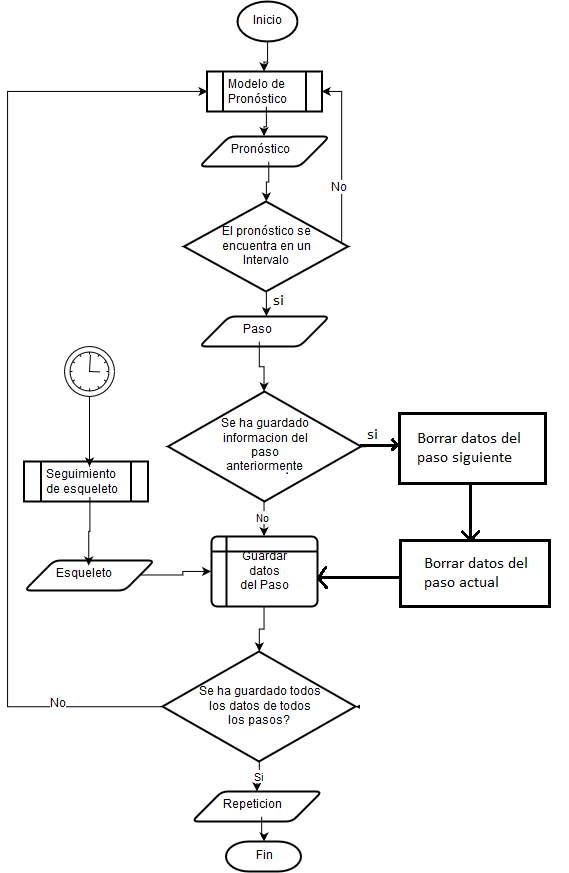
\includegraphics[width=430px,height=470px]{graphics/algoritmoDeteccion.png} \\
	\textbf{Fuente:} Elaborado por el autor de tesis
\end{figure}
\subsection{Validaci\'on del modelo de reconocimiento de movimiento}\label{dis:validate}
El presente proyecto se utiliz\'o dos m\'etodos de validaciones cruzadas \cite{perez2015analisis}:
\begin{itemize}
\item \textbf{Hold out:} La muestra de datos se separa en dos conjunto, uno para construir y entrenar el modelo -i.e. Build- y otro para realizar pruebas que dan validez al error del modelo.
\item \textbf{K-fold:} La muestra se divide en k subconjuntos, y en cada subconjunto se aplica el m\'etodo Hold-out.
\end{itemize}  
\begin{table}[H]
\begin{center}
\caption{Validaci\'on cruzada, 3-fold,  Tenis de mesa}
\label{tab:KfoldTenis}
\begin{tabular}{|l|l|l|}
\hline
\multicolumn{3}{|c|}{\textbf{Muestra de v\'ideos}} \\ \hline
\multicolumn{3}{|c|}{1, 2, 3, 4, 5, 6} \\ \hline
\textbf{Modelo} & \textbf{Builds} & \textbf{Test} \\ \hline
1 & 1, 2, 3, 4, 5 & 6 \\ \hline
2 & 1, 2, 4, 5, 6 & 3 \\ \hline
3 & 2, 3, 4, 5, 6 & 1 \\ \hline
\multicolumn{3}{l}{\textbf{Fuente:} Elaborado por el autor de tesis}
\end{tabular}
\end{center}
\end{table}
\begin{table}[H]
\begin{center}
\caption{Validaci\'on cruzada, 3-fold,  Animaci\'on}
\label{tab:KfoldAnimacion}
\begin{tabular}{|l|l|l|}
\hline
\multicolumn{3}{|c|}{\textbf{Muestra de v\'ideos}} \\ \hline
\multicolumn{3}{|c|}{1, 2, 3, 4, 5, 6, 7} \\ \hline
\textbf{Modelo} & \textbf{Builds} & \textbf{Test} \\ \hline
1 & 1, 2, 3, 4, 5, 6 & 1 \\ \hline
2 & 1, 2, 3, 5, 6, 7 & 4 \\ \hline
3 & 1, 2, 3, 4, 5, 6 & 7 \\ \hline
\multicolumn{3}{l}{\textbf{Fuente:} Elaborado por el autor de tesis}
\end{tabular}
\end{center}
\end{table}
\begin{table}[H]
\begin{center}
\caption{Validaci\'on cruzada, 3-fold,  Taekwondo}
\label{tab:KfoldTaekwondo}
\begin{tabular}{|l|l|l|}
\hline
\multicolumn{3}{|c|}{\textbf{Muestra de videos}} \\ \hline
\multicolumn{3}{|c|}{1, 2, 3, 4, 5, 6, 7, 8, 9, 10, 11, 12, 13, 14, 15, 16} \\ \hline
\textbf{Modelo} & \textbf{Builds} & \textbf{Test} \\ \hline
1 & 1, 2, 3, 4, 5, 6, 7, 8, 9, 11, 12, 13, 14, 15, 16 & 10 \\ \hline
2 & 1, 2, 3, 4, 5, 6, 7, 8, 9, 10, 12, 13, 14, 15, 16 & 11 \\ \hline
3 & 1, 2, 3, 4, 5, 6, 7, 8, 9, 10, 11, 13, 14, 15, 16 & 12 \\ \hline
\multicolumn{3}{l}{\textbf{Fuente:} Elaborado por el autor de tesis}
\end{tabular}
\end{center}
\end{table}
Posteriormente en la etapa de pruebas, se realiz\'o  por cada modelo un hoja de observaciones de valores reales y pron\'onosticados (ver anexo, tabla \ref{tab:obsErrores}), de modo de encontrar los siguientes errores de pron\'osticos \cite{erroresPronostico}:
\begin{itemize}
\item \textbf{Error Medio Pron\'osticado (\acrshort{EMP}):} Promedio de diferencia entre el valor real y pron\'osticado, la cual puede tener tres interpretaciones distintas:
	\begin{itemize}
	\item \textbf{Valor positivo:} En promedio los valores pron\'osticado est\'an por arriba de los valores reales.
	\item \textbf{Valor negativo:} En promedio los valores pron\'osticado est\'an por debajo de los valores reales.
	\item \textbf{Valor cero:} Los valores pron\'osticados pueden estar por debajo o por arriba de los valores reales.
	\end{itemize}
\begin{formula}[H]
	\centering
	\caption{C\'alculo del error medio pron\'osticado}
	\label{frm:empMath}
	\begin{equation}
EMP=\frac{\sum_{0}^{n}(Real_{x}-Pronostic_{x}\cdot10^{-6})}{n}
	\end{equation}
	\textbf{Fuente:} Formula adaptada al proyecto, a partir de la f\'ormula EMP \cite{videoErrores}
\end{formula}  
\item \textbf{Desviaci\'on Media absoluta (\acrshort{DMA}):} Promedio de diferencia absoluta entre el valor real y pron\'osticado, que muestra la dispersi\'on con respecto al valor real.
 \begin{formula}[H]
	\centering
	\caption{C\'alculo de la desviaci\'on media absoluta}
	\label{frm:MADMath}
	\begin{equation}
DMA=\frac{\sum_{0}^{n}( \left |  Real_{x}-Pronostic_{x}\cdot10^{-6} \right |)}{n}
	\end{equation}
	\textbf{Fuente:} Formula adaptada al proyecto, a partir de la f\'ormula DMA \cite{videoErrores}
\end{formula}  
\item \textbf{Ra\'iz del error cuadr\'atico medio (RECM):} Es la desviaci\'on est\'andar de los errores de predicci\'on, la cual indica qu\'e tan disperso se encuentra los errores con respecto al error medio pron\'osticado.
 \begin{formula}[H]
	\centering
	\caption{C\'alculo de la Ra\'iz del error cuadr\'atico medio}
	\label{frm:RECMMath}
	\begin{equation}
RECM=\sqrt{\frac{\sum_{0}^{n}((Real-Pronostic\cdot10^{-6})-EMP)^{2}}{n}}
	\end{equation}
	\textbf{Fuente:} Formula adaptada al proyecto, a partir de la f\'ormula RECM \cite{GEORCMETUT}
\end{formula}  
\end{itemize}
Luego de encontrar los errores, se debe seleccionar el modelo que tenga el menor error \acrshort{RECM}, y posteriormente encontrar los errores de la muestra total:
 \begin{formula}[H]
	\centering
	\caption{EMP de la muestra total}
	\label{frm:EmpAll}
	\begin{equation}
EMP_{muestra\, total}=AVERAGE([EMP_{modelo}])
	\end{equation}
	\textbf{Fuente:} Propuesto por el autor de tesis, en base a las f\'ormulas de excel (versi\'on en ingl\'es)
\end{formula}  
 \begin{formula}[H]
	\centering
	\caption{MAD de la muestra total}
	\label{frm:MadAll}
	\begin{equation}
MAD_{muestra\, total}=AVERAGE([MAD_{modelo}])
	\end{equation}
	\textbf{Fuente:} Propuesto por el autor de tesis, en base a las f\'ormulas de excel (versi\'on en ingl\'es)
\end{formula}  
	 \begin{formula}[H]
	\centering
	\caption{RECM de la muestra total}
	\label{frm:RecmAll}
	\begin{equation}
RECM_{muestra\, total}=AVERAGE([RECM_{modelo}])
	\end{equation}
	\textbf{Fuente:} Propuesto por el autor de tesis, en base a las f\'ormulas de excel (versi\'on en ingl\'es)
\end{formula} 
Los errores de la muestra total ayuda aceptar o rechazar el modelo; si el el error \acrshort{RECM} es menor al valor de identificaci\'on (ver f\'ormula \ref{frm:idenStep}), se aprueba. En caso que sea mayor o igual, se rechaza, debido que existe secciones que no podr\'a identificar el paso, tal como se muestra en la siguiente figura:
\begin{figure}[H]
	\caption{Aprobaci\'on o rechazo del modelo}
	\label{fig:AproveOrDennie}
	\centering
	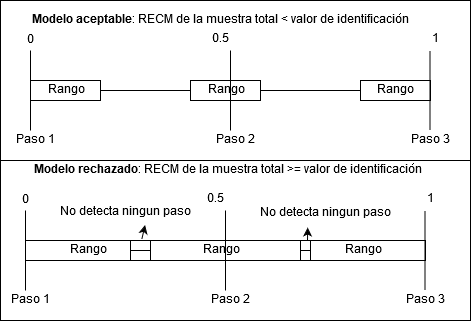
\includegraphics[width=430px,height=180px]{graphics/aceptacionModelo.png} \\
	\textbf{Fuente:} Elaborado por el autor de tesis
\end{figure}
Finalmente, por cada modelo aprobado se debe encontrar el factor de reconocimiento y sus respectivo rango de confiabilidad:
\begin{formula}[H]
	\centering
	\caption{Factor de reconocimiento e intervalos de confianza}
	\label{frm:rangoConfiabilidad}
	\begin{equation}
\begin{matrix}
recognition=\frac{RECM_{muestra\, total}}{valor\: de\: identificacion}  \\ 
\\
intervalo\: de\: confianza = ic =[[inferior,superior]] \\
\\
ic(paso)=\left\{\begin{matrix}
inferior(paso)=\left\{\begin{matrix}
0 & si\, es\, el\, primer\, paso\\ \\ 
etiqueta(paso)-\frac{recognition*valor\, de\, identificacion}{2} & si\: es\: paso\: intermedio \\ 
\\
1-(recognition*valor\, de\, identificacion)& si\, es\, el\, ultimo\, paso
\end{matrix}\right. \\ 
\\ 
inferior(paso)=\left\{\begin{matrix}
recognition*valor\, de\, identificacion& si\, es\, el\, primer\, paso \\
\\
etiqueta(paso)+\frac{recognition*valor\, de\, identificacion}{2} & si\: es\: paso\: intermedio \\ \\ 
1 & si\: es\: el\: ultimo\: paso
\end{matrix}\right.
\end{matrix}\right.
\end{matrix}
	\end{equation}
	\textbf{Fuente:} Propuesto por el autor de tesis
\end{formula} 
\subsection{Dise\~no de los resultados de una rutina tabata} \label{dis:results}
En la presente secci\'on se determina los resultados de la rutina de tabata, dichos resultado son encontrados a partir del seguimiento del esqueleto, la cual proporciona informaci\'on de las variables del detalle de paso y repetici\'on (Ver f\'ormula \ref{frm:MatrizDatosRepeticion}), con el fin objetivo de encontrar la siguiente informaci\'on:
\begin{itemize}
\item \textbf{Volumen de repeticiones:} Sumatoria de las cantidades totales de repeticiones de una serie.  
\begin{code}[H]
	\caption{Pseudoc\'odigo para obtener las repeticiones totales de una rutina}
	\label{code:getRepetitions}
	\begin{lstlisting}
Entrada:
	Series de repeticiones del movimiento
	Contador de Repeticiones

Proceso:
	Recorrer cada serie de repeticiones del movimiento:
		Contar las repeticiones de la serie
		Sumar al contador de repeticiones

Salida
	Contador de repeticiones
	\end{lstlisting}
	\textbf{Fuente:} Elaborado por el autor de tesis
\end{code}

\item \textbf{Duraci\'on:} Tiempo total que se emplea en una rutina, tomando en cuenta todas las series de trabajo y descanso.
\begin{formula}[H]
	\centering
	\caption{c\'alculo de la duraci\'on de tiempo de una rutina}
	\label{eq:DurationTime}
	\begin{equation}
	Duration = \sum_{i=0}^{series}restTime +\sum_{i=0}^{series}workTime = series(restTime+workTime)
	\end{equation}
		\textbf{Fuente:} Elaborado por el autor de tesis
\end{formula}
\item \textbf{Resistencia:} Construye la estructura de la gr\'afica de trabajo de la rutina a partir del recorrido de todas la series, posteriormente en cada serie se recorre todas las repeticiones y luego en cada repetici\'on se almacena el tiempo acumulado de la rutina y la cantidad de repeticiones que lleva el atleta a ese momento.
\begin{code}[H]
	\caption{Pseudoc\'odigo para crear la gr\'afica de resistencia}
	\label{code:getEndurance}
	\begin{lstlisting}
Entrada:
	Series de repeticiones del movimiento
	Grafico, en donde almacena
		Subgrafico, que esta compuesto
			Nombre de la serie
			Listado de puntos, en donde cada punto
				Guarda el tiempo (Eje x)
				Guarda el numero de repeticion (Eje Y)
	
Proceso:
	Crear Grafico
	Recorrer cada serie de repeticiones del movimiento:
		crear subgrafico
		Obtener el numero de serie
		Crear el listado de puntos
		Recorrer cada repeticion de la serie:
			Obtener el numero de repeticion acumulado 
			Obtener el tiempo del paso final de la repeticion (Tiempo)
			Crear un punto
			Guardar punto en el listado de puntos
		Almacenar en el subgrafico el numero de serie y listado de puntos
		Guardar subgrafico en el listado que tiene grafico

Salida
	Grafico de resistencia
	\end{lstlisting}
	\textbf{Fuente:} Elaborado por el autor de tesis
\end{code} 

\item \textbf{Potencia:} Resultado que muestra la cantidad m\'axima de repeticiones en el menor tiempo posible, la cual se encuentra a partir del recorrido de las series, luego en cada serie se determina la cantidad de repeticiones totales y el tiempo acumulado de la \'ultima repetici\'on, encontrando: 
	\begin{itemize}
	\item Una mayor cantidad de repeticiones almacenada anteriormente
	\item La misma cantidad repeticiones almacenada anteriormente, pero se verifica si el tiempo acumulado es menor.
	\end{itemize}
\begin{code}[H]
	\caption{Pseudoc\'odigo para obtener la potencia}
	\label{code:getEndurance}
	\begin{lstlisting}
Entrada
	Series de repeticiones del movimiento
	Potencia, en donde almacena
		Cantidad de repeticiones acumulada de una serie
		Tiempo total de la ultima repeticion de la serie
		
Proceso:
	Crear Potencia
	Recorrer cada serie de repeticiones del movimiento:
		Obtener la ultima repeticion de la serie:
			Obtener el numero de repeticion acumulada
			Obtener el tiempo del paso final de la repeticion
			El numero de repeticiones acumulada aumento?:
				Si:
					Almacenar los datos en potencia
				Sino si: El numero de repeticiones permanecio constante?:
					El Tiempo total se redujo?:
						Almacenar los datos en potencia
						
Salida
	Potencia 
	\end{lstlisting}
	\textbf{Fuente:} Elaborado por el autor de tesis
\end{code} 

\item \textbf{Velocidad}: Raz\'on de cambio separado por:
	\begin{itemize}
	\item \textbf{Repeticiones por serie:} Variable que se determina a partir del promedio total de repeticiones por serie.
		\item \textbf{Tiempo por repeticion:} Variable que se determina a partir del promedio de la diferencia entre el tiempo del paso final y tiempo del paso inicial -i.e. Tiempo de una repetici\'on- de cada repetici\'on realizada por el atleta.
	\end{itemize}
\end{itemize}


\begin{code}[H]
	\caption{Pseudoc\'odigo para obtener las velocidades de las rutinas}
	\label{code:getTimeOfRepetitions}
	\begin{lstlisting}
Entrada
	Series de repeticiones del movimiento
	Velocidad, en donde almacena
		Repeticiones por serie
		Tiempo por serie
		
Proceso:
	Crear Velocidad
	Crear un listado de tiempos de repeticiones
	Crear un listado de repeticiones de series
	Recorrer cada serie de repeticiones del movimiento
		Obtener el total de repeticiones de la serie
		Agregar al listado de repeticiones de series
		Recorrer cada repeticion de la serie
			Obtener el tiempo del paso inicial de la repeticion
			Obtener el tiempo del paso final de la repeticion
			Encontrar la diferencia de tiempos de paso final e inicial
			Almacenar en el listado de tiempos de repeticiones
	Encontrar el promedio de repeticiones de series
	Transformar a numero entero el promedio de repeticiones de series
	Encontrar el promedio de tiempos de repeticiones
	Almacenar ambos promedio en velocidad
	
Salida:
	Velocidad
	\end{lstlisting}
	\textbf{Fuente:} Elaborado por el autor de tesis
\end{code} 
\section{Criterios del proyecto}\label{criter}
En esta secci\'on se presenta todos los criterios que se siguieron para crear el modelo de reconocimientos de movimientos:
\subsection{Criterios de selecci\'on de movimiento}
\begin{itemize}
	\item El investigador y el entrenador de cada deporte,  seleccionaron aquellos movimientos que se ejecutan dentro del \'area de visi\'on del sensor Kinect.
	\item El movimiento no debe ser complejo, es decir que cualquier persona pueda realizar dicho movimiento, sin importar su nivel deportivo.
	\item Debe ser un movimiento que se emplea constantemente en el deporte, para aprender nuevos movimientos complejos.
\end{itemize}
\subsection{Criterios de an\'alisis de movimiento}
\begin{itemize}
	\item Cada movimiento debe tener una articulaci\'on de an\'alisis.
	\item El conjunto de articulaciones que interact\'uan en el movimiento, se debe seleccionar en base a la separaci\'on del cuerpo humano, es decir, la parte inferior (Articulaciones abajo de la cadera central) o superior (Articulaciones arriba de la cadera central).
\end{itemize}
\subsection{Criterios de etiquetaci\'on de movimiento}
\begin{itemize}
	\item Cada repetici\'on del movimiento debe pasar por todos los pasos.
	\item El rango de etiquetaci\'on debe estar entre valores de 0 (Paso inicial) y 1 (Paso final).
	\item La curva de aprendizaje de cada repetici\'on, debe ser similar a la funci\'on Sigmoide -i.e. Gr\'afica con forma de S-.
	\item No se etiqueta los datos de ruidos durante una repetici\'on del movimiento -e.g. Interrupciones, mala ejecuci\'on-.
\end{itemize}
\subsection{Criterios de error del modelo}
\begin{itemize}
	\item Se debe calcular la dispersi\'on entre los datos de la muestra y su media, a partir de la Ra\'iz del error cuadr\'atico medio (RECM).
	\item Se debe calcular la dispersi\'on entre los datos reales y pron\'ositcado a partir de la Desviaci\'on media absoluta (DMA). 
	\item El error se encuentra en un rango de 0 a 1.
\end{itemize}
\subsection{Criterios de selecci\'on del modelo}
\begin{itemize}
	\item Se selecciona el modelo que contenga el menor RECM, en caso que exista RECM iguales, se escoge el modelo que tenga el menor DMA.
\end{itemize}
\subsection{Criterios de aceptaci\'on del modelo}
\begin{itemize}
	\item El modelo seleccionado debe considerar los errores de todas las muestras, a partir del promedio de error de los modelos comparados.
	\item Se aprueba el modelo, s\'i el valor de reconocimiento es menor a 1.
\end{itemize}